\chapter{C++ Basic}

\section{The Birth and Evolution of C++}

Programming languages have always evolved to address the growing complexity of software development. Among these, C++ stands out as a language that bridges the gap between low-level system control and high-level abstraction. It combines the performance of C with the principles of object-oriented programming, enabling developers to tackle complex systems efficiently.

The story of C++ begins with C, a powerful yet simple language created by Dennis Ritchie at Bell Labs in the early 1970s. Its efficiency and portability made it a foundation for system programming. In 1979, Bjarne Stroustrup set out to enhance C by introducing support for object-oriented programming (OOP), creating what he called “C with Classes.” This evolved into C++ in 1983, symbolizing an increment over C, and laid the groundwork for modern software engineering.

Standardization followed in the late 1980s, ensuring compatibility across platforms. Over the years, successive standards like C++11, C++17, and C++20 have introduced features such as smart pointers, lambda expressions, and modules, keeping C++ at the forefront of programming innovation.

\subsection{Key Features of C++}

\begin{itemize}
    \item \textbf{Object-Oriented Programming (OOP)}: 
    C++ introduced core OOP concepts like classes, inheritance, and polymorphism, enabling developers to design modular, reusable, and maintainable software.
    
    \item \textbf{Generic Programming}: 
    The inclusion of templates brought the power of generic programming, allowing for flexible and reusable data structures and algorithms. Techniques like template metaprogramming extended this capability further.
\end{itemize}

\subsection{Modern Applications and Impact}

Today, C++ is used across diverse fields, including game development, embedded systems, scientific computing, and finance. Its combination of performance and expressiveness makes it a vital tool for building software that demands both efficiency and scalability. 

An active open-source community, including projects like the Boost C++ Libraries, has greatly expanded its capabilities. With ongoing innovations like concepts and modules, C++ continues to adapt to the demands of modern software development, ensuring its relevance for decades to come.

\section{The build process}

\subsection{Compiled vs. Interpreted Languages}

\begin{minipage}[H]{0.43\textwidth}
    C++ is a \textbf{compiled language}, which means that the source code must be translated into machine code before it can be executed. This translation process is performed by a \textbf{compiler}, which reads your source code and generates an executable file that can be run on a computer. 
    \vspace{1em}
    \newline
    In contrast, \textbf{interpreted languages} like Python are executed line by line by an \textbf{interpreter}. The interpreter reads the code, evaluates it, and executes the corresponding instructions without generating a separate executable file.
\end{minipage}%
\hspace{0.02\textwidth}% <-- Aggiunge un piccolo spazio tra le minipage
\begin{minipage}[H]{0.55\textwidth}
    \centering
    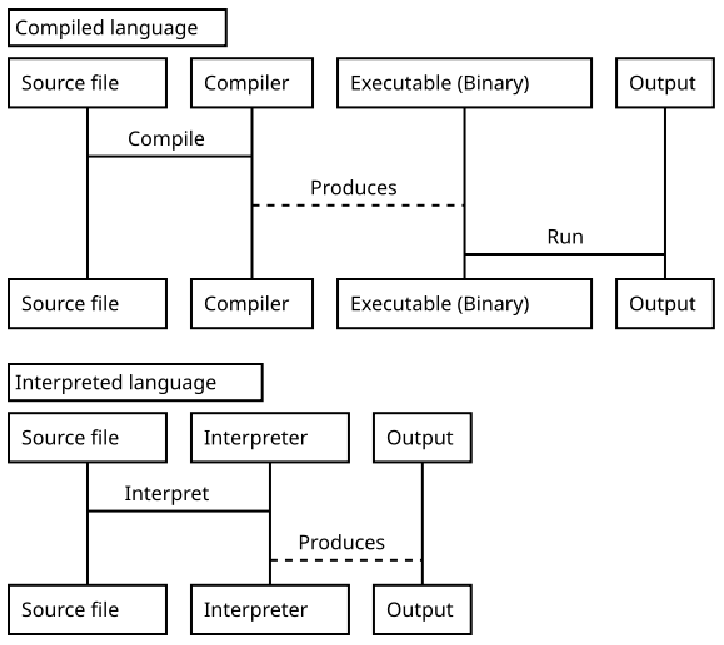
\includegraphics[width=0.8\textwidth]{assets/compiled_vs_interpreted.png}
    \captionof{figure}{Compiled vs. Interpreted Languages}
    \label{fig:compiled_vs_interpreted}
\end{minipage}

\subsection{The Build Process}

The build process for a C++ program involves several steps:

\begin{figure}[H]
    \centering
    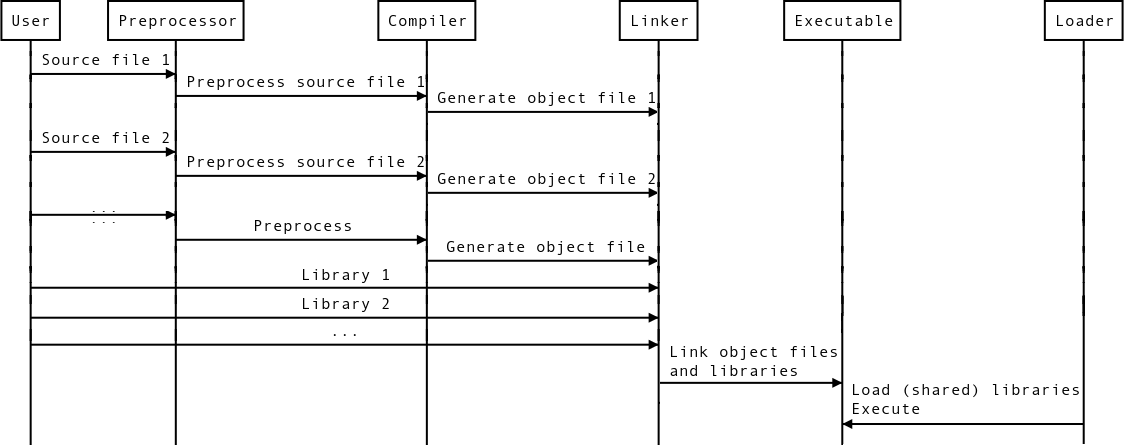
\includegraphics[width=\textwidth]{assets/build_process.png}
    \caption{The Build Process}
    \label{fig:build_process}
\end{figure}

\subsubsection{Preprocessor}

    The preprocessor is the first step in the build process. It processes directives that begin with \texttt{\#} and modifies the source code before it is compiled.
    Common preprocessor directives include:
    
    \begin{itemize}
        \item \texttt{\#include} for including header files;
        \item \texttt{\#define} for defining macros;
        \item \texttt{\#ifdef}, \texttt{\#ifndef}, \texttt{\#else}, \texttt{\#endif} for conditional compilation;
        \item \texttt{\#pragma} for compiler-specific directives.
    \end{itemize}

    \begin{exampleblock}[Preprocessor]
        Original source code:
        
        \begin{codeblock}[language=C++]
    #include <iostream>
    #define GREETING "Hello, World!"
    
    int main() {
        std::cout << GREETING << std::endl;
        return 0;
    }
        \end{codeblock}
        
        Preprocessed source code:
        
        \begin{codeblock}[language=C++]
    // Content of <iostream>, simplified for demonstration
    namespace std {
        extern ostream cout; 
        extern ostream endl;
    }
    
    int main() {
        std::cout << "Hello, World!" << std::endl;
        return 0;
    }
        \end{codeblock}
    \end{exampleblock}    

\subsubsection{Compiler}
    
    The \textbf{compiler} translates the preprocessed source code into assembly or machine code. This phase involves multiple steps:
    \begin{enumerate}
        \item \textbf{Lexical Analysis}: Tokenizes the source code into meaningful elements like keywords, identifiers, and operators.
        \item \textbf{Syntax Analysis (Parsing)}: Constructs a syntax tree or abstract syntax tree (AST) to represent the grammatical structure of the code.
        \item \textbf{Semantic Analysis}: Checks for logical consistency, type compatibility, and adherence to language rules.
        \item \textbf{Code Generation}: Converts the AST into assembly or machine code.
        \item \textbf{Optimization}: Enhances the efficiency of the generated code.
        \item \textbf{Output}: Produces object files containing machine code.
    \end{enumerate}
    
    \begin{neonlisting}[language=bash]{Compiling a C++ File}
g++ main.cpp -o main.o
    \end{neonlisting}
    
    Common compiler options include:
    \begin{itemize}
        \item \texttt{-O}: Specify optimization levels (e.g., \texttt{-O2}, \texttt{-O3}).
        \item \texttt{-g}: Include debugging information for tools like \texttt{gdb}.
        \item \texttt{-std}: Specify the C++ standard (e.g., \texttt{-std=c++17}, \texttt{-std=c++20}).
    \end{itemize}

\subsubsection{Linker}
    
    The \textbf{linker} combines object files into a single executable. This step supports modular programming and ensures that all references between different parts of the program are resolved.
    
    The linking process includes:
    \begin{enumerate}
        \item \textbf{Symbol Resolution}: Matches symbols (function, variable names, ...) between object files.
        \item \textbf{Relocation}: Adjusts memory addresses to create a unified memory layout for the program.
        \item \textbf{Output}: Produces an executable file.
        \item \textbf{Linker Errors/Warnings}: Identifies missing symbols or conflicts.
    \end{enumerate}
    
    \begin{neonlisting}[language=bash]{Linking Object Files}
    g++ main.o helper.o -o my_program
    \end{neonlisting}
    
    Linking can be static or dynamic:
    \begin{itemize}
        \item \textbf{Static Linking}: All required libraries are included in the final binary, resulting in a larger file size. Libraries do not need to be present on the target system.
        \item \textbf{Dynamic Linking}: Libraries are referenced at runtime, resulting in a smaller binary. Requires the necessary libraries to be present on the system during execution.
    \end{itemize}

\subsubsection{Loader}
    
    The \textbf{loader} prepares the executable for execution by loading it into memory, handling these steps:
    \begin{enumerate}
        \item \textbf{Memory Allocation}: Reserves memory for the executable and its data.
        \item \textbf{Relocation}: Adjusts memory addresses as necessary to account for the executable's location in memory.
        \item \textbf{Initialization}: Sets up the runtime environment for the program.
        \item \textbf{Execution}: Begins executing the program's entry point (e.g., \texttt{main()} in C++).
    \end{enumerate}
    
    \begin{observationblock}
        Dynamic linking at runtime enhances flexibility by including external libraries only when the program is executed. This approach reduces the initial binary size and allows for library updates without recompiling the application.
    \end{observationblock}

\section{Structure of a Basic C++ Program}

\subsection{Overview of Program Structure}

A typical C++ program is composed of a collection of functions. Every C++ program must include the \texttt{main()} function, which serves as the entry point. Additional functions can be defined as needed, and their statements are enclosed in curly braces \texttt{\{\}}. Statements are executed sequentially unless control structures like loops or conditionals are applied.

\begin{exampleblock}{Basic Program Structure}
    \begin{codeblock}[language=C++]
#include <iostream>

int main() { // Entry point of the program.
    std::cout << "Hello, world!" << std::endl;
    return 0; // Indicates successful execution.
}
\end{codeblock}

\begin{itemize}
    \item \plaintt{\#include <iostream>}: Includes the Input/Output stream library.
    \item \plaintt{int main()}: The entry point function.
    \item \plaintt{std::cout}: Standard output stream for printing to the console.
    \item \plaintt{<<}: Stream insertion operator.
    \item \plaintt{"Hello, world!"}: The string to print.
    \item \plaintt{<< std::endl}: Outputs a newline character and flushes the stream.
    \item \plaintt{return 0;}: Indicates successful program termination.
\end{itemize}
\end{exampleblock}

\subsubsection{How to Compile and Run}

After writing your C++ program, use the GNU C++ compiler (g++) to create an executable:

\begin{codeblock}[language=bash, numbers=none]
g++ hello_world.cpp -o hello_world
\end{codeblock}

Execute the compiled program from the terminal, optionally passing command-line arguments:

\begin{codeblock}[language=bash, numbers=none]
./hello_world [arg1] [arg2] ... [argN]
\end{codeblock}

Verify the program's execution status by examining its exit code (0 typically indicates success):
\begin{codeblock}[language=bash, numbers=none]
echo $?$
\end{codeblock}

\subsection{C++ as a Strongly Typed Language}

C++ enforces strict type checking during compilation. Variables must be declared with a specific type, ensuring type safety and reducing runtime errors. 

\begin{exampleblock}[Strong Typing in C++]
    \begin{codeblock}[language=C++]
int x = 5;
char ch = 'A';
float f = 3.14;

x = 1.6;        // Legal, but truncated to 1.
f = "a string"; // Illegal.

unsigned int y{3.0}; // Uniform initialization: illegal.
    \end{codeblock}
\end{exampleblock}

\section{Fundamental Types}

C++ provides various built-in types to handle data of different kinds and sizes. These types include integers, floating-point numbers, characters, Booleans, and more.

\begin{table}[H]
    \centering
    \begin{tabular}{|l|c|c|}
        \hline
        \textbf{Data Type} & \textbf{Size (Bytes)} & \textbf{\texttt{<cstdint>}} \\ \hline
        \texttt{bool} & 1 &  \\ \hline
        \texttt{char} & 1 &  \\ \hline
        \texttt{signed char} & 1 & \texttt{int8\_t} \\ \hline
        \texttt{unsigned char} & 1 & \texttt{uint8\_t} \\ \hline
        \texttt{short} & 2 & \texttt{int16\_t} \\ \hline
        \texttt{unsigned short} & 2 & \texttt{uint16\_t} \\ \hline
        \texttt{int} & 4 & \texttt{int32\_t} \\ \hline
        \texttt{unsigned int} & 4 & \texttt{uint32\_t} \\ \hline
        \texttt{long int} & 4 or 8 & \texttt{int32\_t} or \texttt{int64\_t} \\ \hline
        \texttt{long unsigned int} & 4 or 8 & \texttt{uint32\_t} or \texttt{uint64\_t} \\ \hline
        \texttt{long long int} & 8 & \texttt{int64\_t} \\ \hline
        \texttt{long long unsigned int} & 8 & \texttt{uint64\_t} \\ \hline
        \texttt{float} & 4 &  \\ \hline
        \texttt{double} & 8 &  \\ \hline
    \end{tabular}
    \caption{Sizes of Fundamental Types in C++}
\end{table}

\vspace{-2em}
\subsubsection{Integer Numbers}

C++ supports several integer types with varying sizes and value ranges. Common types include \texttt{int}, \texttt{short}, \texttt{long}, and \texttt{long long}.

\begin{exampleblock}{Integer Types} 
    \begin{codeblock}[language=C++]
int age = 30;
short population = 32000;
long long large_number = 123456789012345;
    \end{codeblock}
\end{exampleblock}

\subsubsection{Floating-Point Numbers}

Floating-point types represent real numbers. These include \texttt{float}, \texttt{double}, and \texttt{long double}. They are ideal for representing decimal values.

\begin{exampleblock}{Integer Types}
    \begin{codeblock}[language=C++]
float pi = 3.14;
double gravity = 9.81;
    \end{codeblock}
\end{exampleblock}

\subsubsection{Floating-Point Arithmetic}

Floating-point numbers in C++ are represented using the format $\pm f \cdot 2^e$, where:
\begin{itemize}
    \item $f$: the \textit{significand} or \textit{mantissa}, representing the precision of the number.
    \item $e$: the \textit{exponent}, determining the scale of the number.
    \item $2$: the base, as floating-point numbers are typically stored in binary form.
\end{itemize}

This representation enables efficient handling of very large or very small values but comes with certain limitations, such as rounding errors.

\paragraph{Normalized Numbers:} 
In normalized form, the most significant bit of the significand is always 1, which ensures efficient use of available precision and avoids redundant representations.

\paragraph{IEEE 754 Standard:}
The IEEE 754 Standard defines how floating-point numbers are represented and manipulated. It specifies:
\begin{itemize}
    \item Standardized formats for \texttt{float}, \texttt{double}, and \texttt{long double}.
    \item Rounding rules to maintain accuracy.
    \item Special values such as \texttt{NaN} (Not-a-Number) and infinity for handling exceptional cases.
\end{itemize}


\begin{exampleblock}
    \begin{codeblock}[language=C++]
double epsilon = 1.0;
        
while (1.0 + epsilon != 1.0) {
    epsilon /= 2.0; // Finding machine epsilon.
}
    \end{codeblock}
    \begin{codeblock}[language=C++]
double a = 0.1, b = 0.2, c = 0.3;

if (a + b == c) { // Unsafe comparison.
    // Due to precision limitations, this might not hold true.
}

if (std::abs((a + b) - c) < 1e-9) {
    // Use a tolerance for safe comparison.
}
    \end{codeblock}
\end{exampleblock}



\subsection{Representation of \texttt{NULL}}

\texttt{NULL} is used to represent a null pointer or an invalid memory address. Its representation depends on the system and context:

\begin{itemize}
    \item In C/C++, \texttt{NULL} is typically defined as \texttt{0} or \texttt{(void*)0}.
    \item In memory, a null pointer is often represented by a sequence of \textbf{all-zero bits}. For example:
    \begin{itemize}
        \item On a 32-bit system: \texttt{0x00000000}
        \item On a 64-bit system: \texttt{0x0000000000000000}
    \end{itemize}
    \newpage
    \item Example in C/C++:
\begin{exampleblock}[Representation of NULL]
    \begin{codeblock}[language=C++]
int* ptr = NULL; // ptr points to memory address 0x00000000
if (ptr == NULL) {
    printf("Pointer is NULL\n");
}
    \end{codeblock}
\end{exampleblock}
\end{itemize}

\subsection{Representation of \texttt{NaN}}

\texttt{NaN} (Not a Number) is a special value used in floating-point arithmetic to represent undefined or unrepresentable results. Its representation is defined by the \textbf{IEEE 754 floating-point standard}:

\begin{itemize}
    \item A \texttt{NaN} value is represented by an \textbf{exponent filled with 1s} (all bits set to 1) and a \textbf{non-zero significand}.
    \item There are two types of \texttt{NaN}:
    \begin{itemize}
        \item \textbf{Quiet NaN (qNaN)}: Used for undefined or unrepresentable results. It has a leading \texttt{1} in the significand.
        \item \textbf{Signaling NaN (sNaN)}: Used to trigger exceptions in certain operations. It has a leading \texttt{0} in the significand.
    \end{itemize}
    \item Example in C/C++:
\begin{exampleblock}[Representation of NaN]
    \begin{codeblock}[language=C++]
#include <cmath>
#include <cstdio>

int main() {
    double result = 0.0 / 0.0; // Results in NaN
    if (isnan(result)) {
        printf("Result is NaN\n");
    }
    return 0;
}
    \end{codeblock}
\end{exampleblock}

\end{itemize}

\subsection{Key Differences}

\begin{tabular}{|l|l|l|}
    \hline
    \textbf{Feature} & \textbf{\texttt{NULL}} & \textbf{\texttt{NaN}} \\ \hline
    Purpose & Represents a null pointer & Represents an undefined floating-point value \\ \hline
    Data Type & Used with pointers & Used with floating-point numbers \\ \hline
    Representation & All-zero bits (e.g., \texttt{0x00000000}) & Exponent filled with 1s and non-zero significand \\ \hline
    Context & Memory addresses, pointers & Floating-point arithmetic \\ \hline
\end{tabular}

\subsubsection{Characters and Strings}

Characters in C++ are represented using the \texttt{char} type, while strings are sequences of characters represented by the \texttt{std::string} class.

\begin{exampleblock}[Working with Characters and Strings]
    \begin{codeblock}[language=C++]
char letter = 'A'; // Single character.
std::string name = "Alice"; // String of characters.
std::string greeting = "Hello, " + name + "!"; // Concatenation.
    \end{codeblock}
\end{exampleblock}

\subsubsection{Boolean Types}

C++ provides a built-in \plaintt{bool} type for logical values. A \texttt{bool} variable can hold one of two values, \texttt{true} or \texttt{false}, useful for conditional statements and logical operations.

Note that numbers can be implicitly converted to \texttt{bool}: 0 is \texttt{false}, while any other value is \texttt{true}.

\begin{exampleblock}[Boolean]
    \begin{codeblock}[language=C++]
bool is_happy = true;
bool is_sad = false;

if (is_happy) {
    std::cout << "You are happy!" << std::endl;
}
    \end{codeblock}
    \begin{codeblock}[language=C++]
if (-1.5) // true
if (0)    // false
    \end{codeblock}
\end{exampleblock}

\subsubsection{Initialization and Aliases}

Initialization assigns an initial value to a variable at the time of declaration. C++ supports several initialization methods: direct, copy, and uniform initialization.

\textbf{Type Aliases} can create alternative names for existing types using \texttt{using} or \texttt{typedef}.

\begin{exampleblock}[Initialization and Type Aliases]
    Variable Initialization:
    \begin{codeblock}[language=C++]
        int x = 42;     // Direct initialization.
        int y(30);      // Constructor-style initialization.
        int z{15};      // Uniform initialization (preferred).
    \end{codeblock}
    Type Aliases:
    \begin{codeblock}[language=C++]
        using integer = int;    // Alias for int.
        integer count = 100;
        
        typedef float distance; // Alias for float.
        distance meters = 250.5;
    \end{codeblock}
\end{exampleblock}



\newpage

\subsection{The \plaintt{auto} Keyword and Type conversion}

The \texttt{auto} keyword allows the compiler to deduce the type of a variable based on its initialization value. This is useful for simplifying code and avoiding verbose type declarations.

\begin{exampleblock}[The \plaintt{auto} Keyword]
    \begin{codeblock}[language=C++]
auto a{42};         // int.
auto b{12L};        // long.
auto c{5.0F};       // float.
auto d{10.0};       // double.
auto e{false};      // bool.
auto f{"string"};   // char[7].
    \end{codeblock}
\end{exampleblock}

\begin{tipsblock}[Best Practices]
    \begin{itemize}
        \item Use \plaintt{auto} for complex types or when the exact type is unimportant.
        \item Avoid \plaintt{auto} for publicly visible variables or ambiguous initializations.
    \end{itemize}
\end{tipsblock}

C++ supports \textbf{implicit and explicit type conversions} to convert between different data types. Implicit conversions are performed automatically by the compiler, while explicit conversions require manual intervention.

\begin{exampleblock}[Type Conversion]
    Implicit conversion:
    \begin{codeblock}[language=C++]
int x = 10;
double y = x; // int to double (implicit).
    \end{codeblock}
    Explicit conversion:
    \begin{codeblock}[language=C++]
double z = 3.14;
int w = static_cast<int>(z); // double to int (explicit).
    \end{codeblock}
\end{exampleblock}

\section{Memory Management}

In computer programming, memory is divided into two main regions: the \textbf{stack} and the \textbf{heap}. These regions serve different purposes and are managed differently. Below is a detailed explanation of their differences.

\subsection{Stack Memory}

The \textbf{stack} is used for \textbf{static memory allocation}, where memory is allocated and deallocated in a last-in, first-out (LIFO) order.

\subsubsection{Key Characteristics of Stack Memory}
\begin{itemize}
    \item \textbf{Purpose}: Used for storing local variables, function parameters, and return addresses.
    \item \textbf{Management}: Memory allocation and deallocation are handled automatically by the compiler.
    \item \textbf{Speed}: Accessing the stack is very fast because it uses a simple pointer-based mechanism (the stack pointer).
    \item \textbf{Size}: The stack has a limited size, which is determined at the start of the program. If the stack exceeds its size, a \textbf{stack overflow} occurs.
    \item \textbf{Lifetime}: Memory is automatically freed when the function or block that allocated it exits.
    \item \textbf{Fragmentation-Free}: The stack does not suffer from fragmentation because memory is always allocated and freed in a strict order.
\end{itemize}


\begin{exampleblock}[Stack Memory Example]
    \begin{codeblock}[language=C++]
void foo() {
    int x = 10; // 'x' is allocated on the stack
    // Memory for 'x' is automatically freed when 'foo' exits
}
    \end{codeblock}
\end{exampleblock}

\subsection{Heap Memory}

The \textbf{heap} is used for \textbf{dynamic memory allocation}, where memory can be allocated and deallocated in any order.

\subsubsection{Key Characteristics of Heap Memory}
\begin{itemize}
    \item \textbf{Purpose}: Used for dynamically allocated data (e.g., arrays, objects, or data structures whose size is not known at compile time).
    \item \textbf{Management}: Memory allocation and deallocation are managed manually by the programmer (e.g., using \texttt{malloc}/\texttt{free} in C or \texttt{new}/\texttt{delete} in C++).
    \item \textbf{Speed}: Accessing the heap is slower than the stack because it involves more complex memory management.
    \item \textbf{Size}: The heap is much larger than the stack and can grow dynamically as needed (limited only by the system's available memory).
    \item \textbf{Lifetime}: Memory remains allocated until it is explicitly freed by the programmer. If not freed, it leads to \textbf{memory leaks}.
    \item \textbf{Fragmentation}: The heap can suffer from fragmentation over time, as memory is allocated and freed in arbitrary order.
\end{itemize}

\begin{exampleblock}[Heap Memory Example]
    \begin{codeblock}[language=C++]
void bar() {
    int* ptr = new int(20); // 'ptr' points to memory allocated on the heap
    // Memory for 'ptr' must be explicitly freed
    delete ptr; // Free the memory to avoid a memory leak
}
    \end{codeblock}
\end{exampleblock}

\subsection{Key Differences Between Stack and Heap}

\begin{tabular}{|l|l|l|}
    \hline
    \textbf{Feature} & \textbf{Stack Memory} & \textbf{Heap Memory} \\ \hline
    Purpose & Static memory allocation & Dynamic memory allocation \\ \hline
    Management & Automatic (compiler-managed) & Manual (programmer-managed) \\ \hline
    Speed & Very fast & Slower \\ \hline
    Size & Limited (predefined size) & Large (limited by system memory) \\ \hline
    Lifetime & Automatically freed when scope ends & Must be explicitly freed \\ \hline
    Fragmentation & No fragmentation & Can suffer from fragmentation \\ \hline
    Usage & Local variables, function parameters & Dynamically allocated data \\ \hline
\end{tabular}

\subsection{When to Use Stack vs. Heap}

\begin{itemize}
    \item \textbf{Use the Stack}:
    \begin{itemize}
        \item For small, short-lived data (e.g., local variables, function parameters).
        \item When the size of the data is known at compile time.
        \item When you want fast and automatic memory management.
    \end{itemize}
    \item \textbf{Use the Heap}:
    \begin{itemize}
        \item For large or dynamically sized data (e.g., arrays, objects).
        \item When the lifetime of the data extends beyond the current scope.
        \item When you need flexibility in memory allocation and deallocation.
    \end{itemize}
\end{itemize}

\subsection{Variables and Pointers}

Variables represent named memory locations, while pointers store memory addresses, enabling direct access and manipulation.
\textbf{Stack Variables} are declared locally within functions or blocks, are stored on the stack and are accessible directly.
\textbf{Heap Variables} require pointers for access and explicit deallocation.

\begin{exampleblock}[Working with Variables and Pointers]
    \begin{codeblock}[language=C++]
int value = 10;       // Stack variable
int* ptr = &value;    // Pointer to stack variable

int* heap_var = new int(25); // Pointer to heap-allocated variable
*heap_var = 30;       // Modify heap variable through pointer

// Cleanup
delete heap_var;      // Deallocate heap memory
heap_var = nullptr;   // Reset pointer.
    \end{codeblock}
\end{exampleblock}

\subsection{Lifetime and Scope}

The lifetime of a variable refers to the duration it exists in memory, while its scope defines where it is accessible in code.

\textbf{Stack Variables}
\begin{itemize}
    \item Limited to the scope of their defining function or block.
    \item Automatically deallocated when the scope ends.
\end{itemize}

\textbf{Heap Variables}
\begin{itemize}
    \item Persist beyond their defining scope until explicitly deallocated.
    \item Risk memory leaks if not deallocated properly.
\end{itemize}

\begin{exampleblock}[Lifetime and Scope Example]
    \begin{codeblock}[language=C++]
void example() {                  //        Lifetime:
    int stack_var = 5;            // ends with the function.
    int* heap_var = new int(10);  // persists until delete.

    delete heap_var;              // Deallocate heap memory.
    heap_var = nullptr;           // Reset pointer.
}
    \end{codeblock}
\end{exampleblock}

\begin{tipsblock}[Best Practices for Memory Management]
    \begin{itemize}
        \item Use stack memory for small, short-lived variables.
        \item Use heap memory for large or long-lived data.
        \item Always match \plaintt{new} with \plaintt{delete} and \plaintt{new[]} with \plaintt{delete[]}.
        \item Prefer modern alternatives like \plaintt{std::unique\_ptr} or \plaintt{std::shared\_ptr} to manage heap memory safely.
    \end{itemize}
\end{tipsblock}

\Large To be continued... \normalsize

\newpage

\section{The Build toolchain in practice}

\subsection{Preprocessor and Compiler}

The build process starts with the \textbf{preprocessor} (\texttt{cpp}) and the \textbf{compiler} (\texttt{g++}, \texttt{clang++}):
\begin{itemize}
    \item \textbf{Preprocessor}: Handles directives like \texttt{\#include}, performs macro substitution, and prepares code.
    \item \textbf{Compiler}: Translates preprocessed code into machine-readable object files.
    \end{itemize}

These steps are often combined when using a compiler command like \texttt{g++} or \texttt{clang++}.

\begin{exampleblock}[Preprocessor and Compiler]
    For a project with three files (\plaintt{module.hpp}, \plaintt{module.cpp}, \plaintt{main.cpp}), the following commands illustrate preprocessing and compilation:
    
    \begin{codeblock}[language=bash, numbers=none]
# Preprocessor step.
g++ -E module.cpp -I/path/to/include/dir -o module_preprocessed.cpp
g++ -E main.cpp -I/path/to/include/dir -o main_preprocessed.cpp

# Compilation step.
g++ -c module_preprocessed.cpp -o module.o
g++ -c main_preprocessed.cpp -o main.o
    \end{codeblock}
\end{exampleblock}

\subsection{Linker}

The \textbf{linker} (\texttt{ld}) combines object files into an executable program by resolving external references between them. It also links external libraries if required.

\begin{exampleblock}[Linker]
    \begin{codeblock}[language=bash, numbers=none]
g++ module.o main.o -o my_program
    \end{codeblock}
\end{exampleblock}

\textbf{Linking Against Libraries}

To link against external libraries, use the \texttt{-l} flag for library names (without the \texttt{lib} prefix or file extension) and the \texttt{-L} flag to specify the library directory:

\begin{codeblock}[language=bash, numbers=none]
g++ module.o main.o -o my_program -lmy_lib -L/path/to/my/lib
\end{codeblock}

The \texttt{-lmy\_lib} flag links to the \texttt{libmy\_lib.so} (dynamic) or \texttt{libmy\_lib.a} (static) file in the specified directory.

\subsection{Preprocessor, Compiler, Linker: Simplified Workflow}

For small projects with few dependencies, a single command can handle preprocessing, compilation, and linking:

\begin{codeblock}[language=bash, numbers=none]
g++ mod1.cpp mod2.cpp main.cpp -I/path/to/include/dir -o my_program
\end{codeblock}

\begin{warningblock}[Compiler Behavior]
Different compilers (e.g., GCC, Clang) may produce varying behaviors, warnings, or errors. For an example of such differences, see this comparison on \href{https://godbolt.org/z/1M83E4sYE}{GodBolt}.
\end{warningblock}

\subsection{Loader}

The \textbf{loader} is responsible for preparing the executable program for execution:
\begin{itemize}
    \item Allocates memory for code and data sections.
    \item Resolves addresses for dynamically linked libraries.
    \item Starts program execution.
\end{itemize}

\textbf{Running an Executable}

\begin{codeblock}[language=bash, numbers=none]
./my_program
\end{codeblock}

\textbf{Dynamic Libraries and \texttt{LD\_LIBRARY\_PATH}}

When linking against external dynamic libraries, the loader uses the environment variable \texttt{LD\_LIBRARY\_PATH} to locate them. Ensure the required library paths are included:

\begin{codeblock}[language=bash, numbers=none]
export LD_LIBRARY_PATH+=:/path/to/my/lib
./my_program
\end{codeblock}
